% ncse_new/p2_InterpolationApproximation/ch1_PolynomialInterpolation/ex_ChebIntp2.tex
% exercise requires:    -
% solutions require:    adaptivepolyintp.m  plot_adaptivepolyintp.m  plot_adaptivepolyintp.eps


\begin{problem}[Adaptive polynomial interpolation]\label{prb:ChebIntp2}

In \ncsesect{sec:ChebychevInterpolation} we have seen that the placement of
interpolation nodes is key to a good approximation by a polynomial
interpolant. The following \emph{greedy algorithm} attempts to find the location
of suitable nodes by its own:
\begin{quote}
  Given a function $f:[a,b]\mapsto \bbR$ one starts
  $\Ct:=\{\frac{1}{2}(b+a)\}$. Based on a fixed finite set
  $\Cs\subset[a,b]$ of \emph{sampling points} one augments the set of nodes
  according to
  \begin{gather}
    \label{rb:1}
    \Ct = \Ct \cup \left\{\operatorname*{argmax}\limits_{t\in\Cs}
    |f(t)-\Op{I}_{\Ct}(t)|\right\}\;,
  \end{gather}
  where $\Op{I}_{\Ct}$ is the polynomial interpolation operator for
  the node set $\Ct$, until 
  \begin{gather}
    \label{rb:2}
    \operatorname*{max}\limits_{t\in\Cs}
   |f(t)-\Op{I}_{\Ct}(t)| \leq \mathtt{tol}\cdot 
   \operatorname*{max}\limits_{t\in\Cs}
    |f(t)|\;.
  \end{gather}
\end{quote}

% ============== SUBPROBLEM 1

\begin{subproblem}[3]\label{subprb:ChebIntp2_1}
Write a MATLAB function 
\begin{center}
  \texttt{function t = adaptivepolyintp(f,a,b,tol,N)}
\end{center}
that implements the algorithm described above and takes as arguments the function
handle \texttt{f}, the interval bounds \texttt{a}, \texttt{b}, the
relative tolerance \texttt{tol}, and the number \texttt{N} of 
\emph{equidistant} sampling points (in the interval $[a,b]$), that is,
\begin{gather*}
  \Cs := \{a+(b-a)\frac{j}{N},\;j=0,\ldots,N\}\;.
\end{gather*}

\begin{hint}
The function \texttt{intpolyval} from \ncseref[Code]{barycentricformula}
is provided and may be used (though it may not be the most efficient way
to implement the function).
\end{hint}

\begin{solution}
See \autoref{mc:ChebIntp2_adaptivepolyintp}.
\end{solution}
\end{subproblem}

% ============== SUBPROBLEM 2

\begin{subproblem}[2]\label{subprb:ChebIntp2_2}
Extend the function from the previous sub-problem so that it
reports the quantity 
\begin{gather}
\label{AIP:1}
\operatorname*{max}\limits_{t\in\Cs}
|f(t)-\Op{T}_{\Ct}(t)| % \leq \mathtt{tol}
\end{gather}
for each intermediate set $\Ct$. 

\begin{solution}
See \autoref{mc:ChebIntp2_adaptivepolyintp}.
%
\lstinputlisting[caption={Implementation of the function \texttt{adaptivepolyintp}},label={mc:ChebIntp2_adaptivepolyintp}]
{\problems/ch_polynomialinterpolation/MATLAB/adaptivepolyintp.m}
\end{solution}
\end{subproblem}

% ============== SUBPROBLEM 3

\begin{subproblem}[2]\label{subprb:ChebIntp2_3} 
For $f_{1}(t) :=
\sin(e^{2t})$ and $f_{2}(t) = \frac{\sqrt{t}}{1+16t^{2}}$ plot the quantity from
\eqref{AIP:1} versus the number of interpolation nodes. Choose plotting styles
that reveal the qualitative decay of this error as the number of interpolation
nodes is increased. Use interval $[a,b] = [0,1]$, \texttt{N=1000} sampling points,
tolerance \texttt{tol = 1e-6}.

\begin{solution}
See \autoref{mc:ChebIntp2_plot_adaptivepolyintp} and \autoref{fig:ChebIntp2_plot_adaptivepolyintp}.
%
\lstinputlisting[caption={Implementation of the function \texttt{plot\_adaptivepolyintp}},label={mc:ChebIntp2_plot_adaptivepolyintp}]
{\problems/ch_polynomialinterpolation/MATLAB/plot_adaptivepolyintp.m}
%
\begin{figure}
\centering
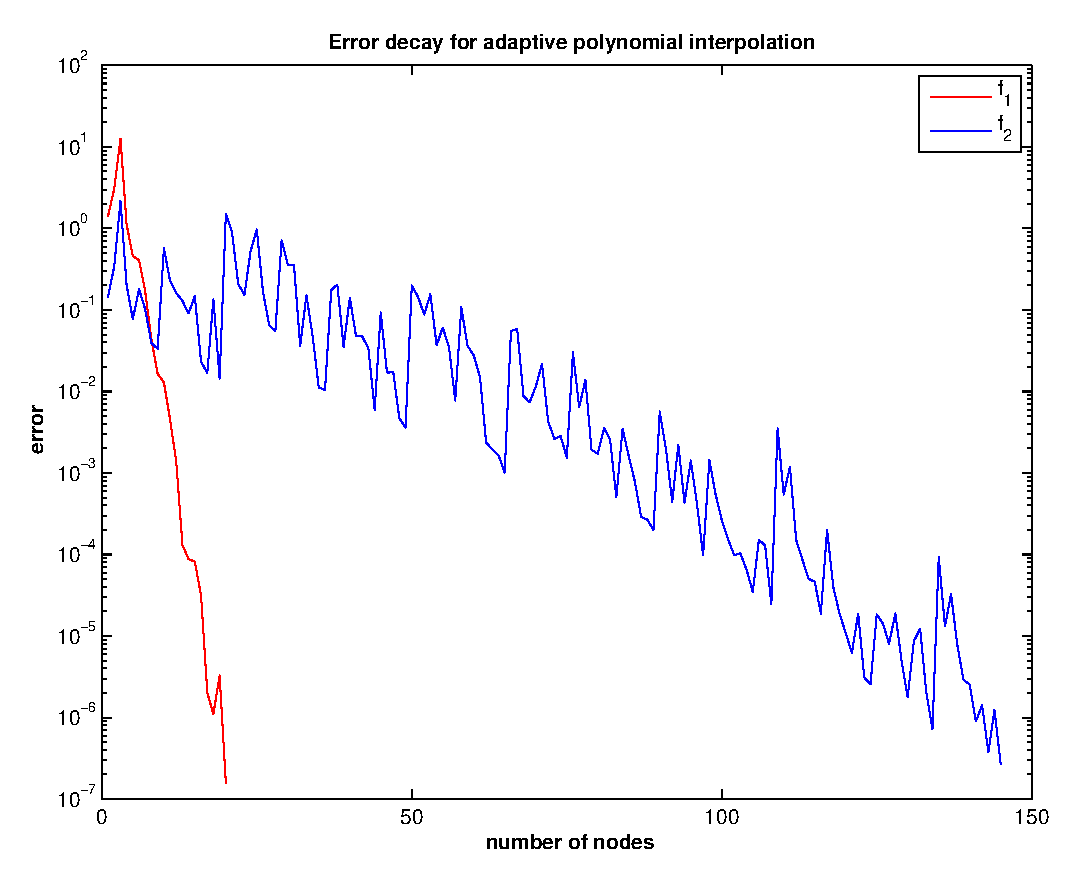
\includegraphics[width=0.7\textwidth]{\problems/ch_polynomialinterpolation/PICTURES/plot_adaptivepolyintp.eps}
\caption{The quantity from \eqref{AIP:1}
versus the number of interpolation nodes.}
\label{fig:ChebIntp2_plot_adaptivepolyintp}
\end{figure}
\end{solution}
\end{subproblem}
\end{problem}
